\section{Processi di supporto}
\subsection{Documentazione}

\subsubsection{Scopo}
Tutti i processi e le attività di sviluppo necessitano di essere documentate. In questa sezione vengono riportate le convenzioni e le norme da applicare in fase di stesura e tutti gli strumenti di cui i componenti del Team Oberon hanno bisogno.
\subsubsection{Aspettative}
\begin{itemize}
    \item Definire una struttura chiara che renda i documenti uniformi tra loro;
    \item Avere delle norme da seguire per ogni aspetto della stesura del documento, in modo da rendere capace di lavorare in modo autonomo ogni componente del gruppo;
\end{itemize}
\subsubsection{Descrizione}
La documentazione è essenziale per tenere traccia di tutte le informazioni relative alle attività svolte e alle decisioni prese durante lo svolgimento del progetto. Grazie ad essa, tutti gli stakeholder possono avere un resoconto del lavoro.
\subsubsection{Ciclo di vita del documento}
\begin{enumerate}
    \item Pianificazione: durante una prima fase di brain storming i componenti del gruppo raccolgono tutte le idee per la creazione del documento e vengono definite le parti che lo compongono;
    \item Impostazione: viene prodotta una prima bozza del documento e il suo scheletro;
    \item Realizzazione: il contenuto del documento viene redatto;
    \item Verifica: il documento è sottoposto ad un’attenta revisione per individuare e correggere eventuali errori;
    \item Approvazione: l’approvatore dà il suo consenso al documento, perciò è completo e pronto per il rilascio;
\end{enumerate}

\subsubsection{Stile Generale}
Il materiale contenuto nei vari documenti sarà preferibilmente riassuntivo, non eccessivamente formale e di semplice comprensione e fruizione, saranno valorizzati grafici e schemi per facilitare e velocizzare l’acquisizione delle informazioni.  \newline
Per la creazione dei documenti di progetto verrà utilizzato il markup language LaTeX basando ogni istanza su un template predeterminato.

\subsubsection{Intestazione}
\begin{enumerate}
    \item Ogni documento redatto dal gruppo avrà una pagina introduttiva contenente il logo, seguito dal titolo, dalla versione e dai componenti del gruppo. Infine conterrà il link alla repository GitHub.
    \item La pagina successiva sarà interamente dedicata al registro delle modifiche degne di nota in un’apposita tabella, con le seguenti colonne: versione, data, nominativo, ruolo, descrizione dell'aggiornamento.
    \item  Infine, la terza e ultima pagina dell'intestazione conterrà il sommario LaTeX che si aggiornerà all'aggiunta di ogni sezione.
\end{enumerate}

\subsubsection{Template}
Il team Oberon ha deciso di adottare un template in modo tale da aver ben definito la struttura base dei documenti.\\
Questo facilità di gran lunga la creazione e il mantenimento di nuovi documenti, infatti l'aspetto e la struttura base viene definito a priori.\\
Questo include il frontespizio, il registro delle modifiche e l'indice.\\\\
Informazioni riportate in:
\\\\
\textbf{Frontespizio}
\begin{itemize}
\setlength\itemsep{0em}
    \item nome del documento
    \item anno accademico
    \item dati relativi ai componenti del gruppo
    \item indirizzo della repository di GitHub
\end{itemize}

\textbf{Registro delle modifiche}
\begin{itemize}
\setlength\itemsep{0em}
    \item Versione: il formato della versione è del tipo x.y.z dove x è il numero della versione approvata per la revisione
    \item Data: il formato è DD/MM/YY
    \item Nominativo: colui che ha modificato il documento
    \item Ruolo: descrive il ruolo principale assunto nello scrum attuale
    \item Descrizione: breve descrizione sulle modifiche effettuate
\end{itemize}

\textbf{Indice norme di progetto}\\
L'indice è autogenerato ed è suddiviso il tre sezioni principali:
\begin{itemize}
\setlength\itemsep{0em}
    \item processo primario
    \item processo di supporto
    \item processo organizzativo
\end{itemize}
Ad ogni sezione è associata al tutte le norme correlate da seguire per mantenere un approccio sistematico, disciplinato e quantificabile allo sviluppo.

\subsubsection{Uso del template}
Per le modifiche dei progetti è fortemente consigliato seguire la seguente procedura:
\begin{enumerate}
    \item Scaricare la cartella Template Latex in formato .zip
    \item Importare la cartella compressa su Overleaf (Nuovo Progetto --> Carica Progetto --> Upload .zip file)
    \item Andare su Menu (in alto a sinistra) --> Documento Principale e settare main.tex
    \item Modificare il titolo del documento in main.tex
    \item Creare un file sezioneX.tex per ogni sezione e importarlo in main.tex
    \item Aggiornare import.tex su GitHub se modificato
    
    \item Una volta finito il documento, la cartella da caricare su GitHub dovrà contenere: \begin{itemize}
        \item main.tex del documento
        \item files sezioneX.tex del documento
        \item pdf esportato del documento
    \end{itemize}
    
\end{enumerate}

\subsubsection{Struttura Glossario}
Il glossario è un semplice documento che raggruppa i termini utilizzati nella stesura degli altri documenti affiancandoli alle loro definizioni, questo facilita la comprensioni di chiunque degli argomenti trattati. \\ La sua struttura è basilare, si limita ad ordinare alfabeticamente una serie di piccole descrizioni delle varie parole chiave del progetto.

\subsubsection{Struttura Piano di Qualifica}

Il piano di qualifica descrive tutti i mezzi adottati per misurare e monitorare sia la qualità dei processi (primari, secondari e organizzativi) che quella del software.\\
La qualità del prodotto è descritto attraverso metriche che hanno come obiettivo garantire certe qualità del software rispettandole.\\
Le metriche e gli obiettivi sono descritti in formato tabellare.\\
I valori delle metriche variano nel tempo e il loro andamento sono descritti come grafici.\\
Inoltre nella parte conclusiva del documento sono riportati tutti i test necessari da superare per raggiungere la maturità del prodotto.


\subsubsection{Struttura Rendiconto delle ore}
Sia il preventivo che il consuntivo delle ore rendicontate di lavoro vengono registrati sui rispettivi file Excel su Teams.
\subsubsection*{Preventivo}
Il preventivo è suddiviso in vari fogli (2 per scrum):
\begin{itemize}
    \item il primo contiene le ore che il team prevede di dedicare ad ogni ruolo per membro;
    \item il secondo contiene lo stato delle ore totali al momento della compilazione (la somma del consuntivo precedente e del preventivo attuale).
\end{itemize}
\subsubsection*{Consuntivo}
Il consuntivo è suddiviso in vari fogli (2 per scrum):
\begin{itemize}
    \item il primo contiene le ore che il team ha effettivamente dedicato ad ogni ruolo per membro;
    \item il secondo contiene lo stato delle ore totali al momento della compilazione (la somma totale dei consuntivi finora). Questo permette di tenere bene traccia dell'andamento del progetto.
\end{itemize}
Le tabelle prodotte ad ogni scrum vengono poi incorporate nel piano di progetto.

\subsubsection{Struttura Piano di Progetto}

Il piano di progetto è suddiviso in tre sezioni principali:

\begin{itemize}
    \item Analisi dei rischi
    \item Pianificazione
    \item Bilancio
\end{itemize}

\begin{center}
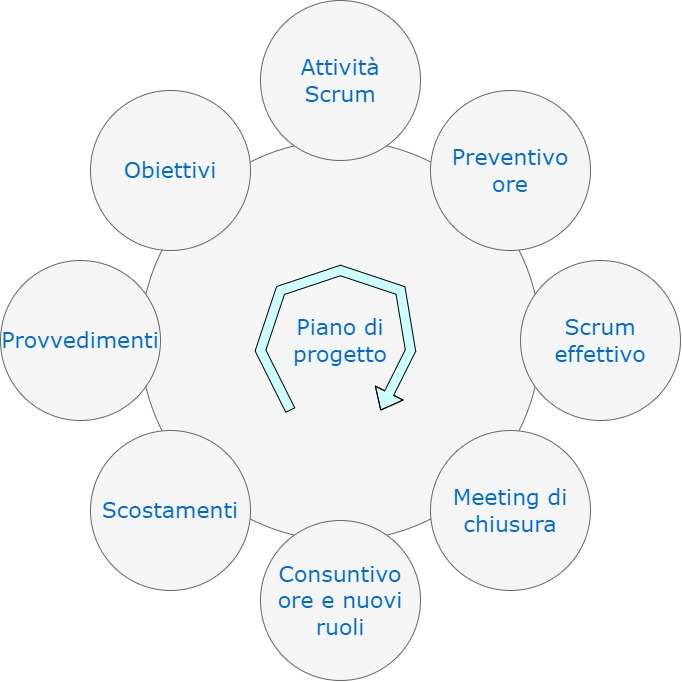
\includegraphics[scale = 0.40]{img/workflow.jpg}
\end{center}

\subsubsection{Analisi dei rischi}

L'analisi dei rischi serve a prevenire e mitigare futuri imprevisti in modo tale da reagire con decisioni ragionevoli in tempi brevi.\\
Il grado di rischio considera sia la frequenza che la gravità dell'evento analizzato.\\
I rischi possono essere di natura umana e di carattere tecnologico.\\
Il piano di contigenza ordina i rischi in base al grado e descrive in modo sintetico le procedure da seguire che portano a risultati concreti.\\
Ogni qualvolta che si verifica un'evento, se è presente nella lista degli eventi considerati si seguono le procedure e viene riportato il riassunto di ciò che si fatto nell'attualizzazione, altrimenti si aggiorna la tabella dei rischi e si ragiona un piano di contigenza adatto per futuri episodi.\\

\begin{center}
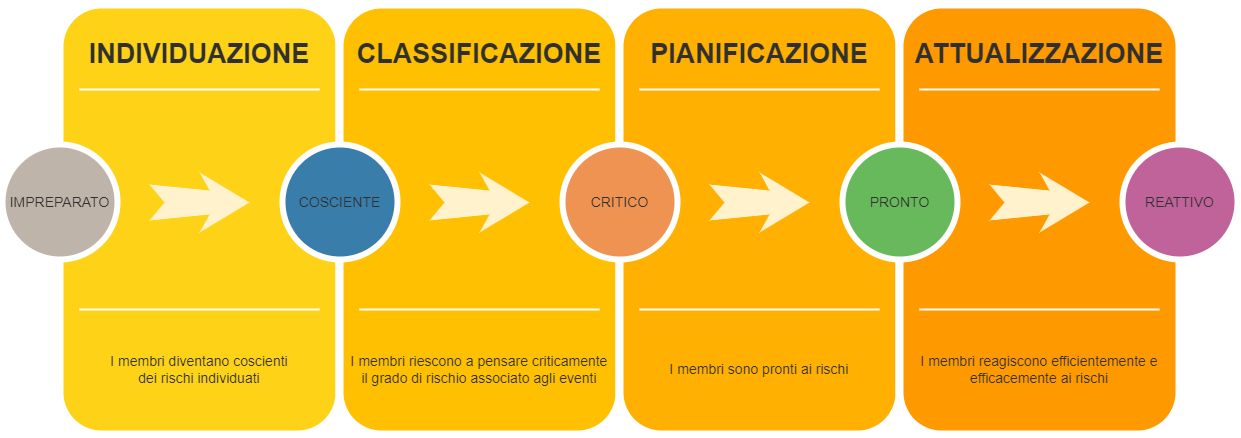
\includegraphics[scale=0.3]{img/analisi_rischi.png}
\end{center}

\subsubsection{Documentazione Scrum}
\begin{enumerate}
    \item Product Backlog, il documento che contiene la lista di tutti requisiti necessari per la realizzazione del progetto, la sua prima stesura definisce i requisiti inizialmente conosciuti, per poi evolversi in base a come evolve il prodotto, ai feedback ricevuti dal cliente e alle necessità che emergono; 
    \item Sprint Backlog, è l’insieme degli elementi del Product Backlog selezionati per lo sprint, è una previsione fatta dal Team in relazione alle priorità indicate e al lavoro necessario per raggiungere gli obiettivi dello sprint; 
    \item Incremento, è la somma di tutti gli elementi del Product Backlog completati durante uno sprint.
\end{enumerate}

\subsubsection{Struttura verbali}
\begin{itemize}
    \item Dati introduttivi: titolo verbale numerato ordinalmente a partire dal primo di quella categoria (es. incontri con il proponente, scrum review…), luogo, data, durata, partecipanti (per il gruppo è sufficiente indicare “membri del team Oberon”);
    \item Sezione Informazioni Generali: breve resoconto degli argomenti trattati nell'incontro descritto dal verbale, utile a chi è alla ricerca di un’informazione in particolare e consulta in velocità questa sezione; 
    \item Sezione Resoconto: nucleo del documento, qui verranno indicati tutti gli argomenti discussi in dettaglio e le conclusioni alle quali si è giunti.

\end{itemize}

\subsubsection{Nomi file}
\textbf{Verbali}: il nome di ogni verbale avrà la seguente struttura "\textit{TipologiaVerbale\_YYYY\_MM\_DD}" dove \textit{TipologiaVerbale} potrà essere: \textit{VerbaleInterno} per i verbali di incontri interni tra i membri del Team Oberon, \textit{VerbaleEsterno} per i verbali di incontri con il proponente di C2, \textit{Verbale\_N\_Scrum} per i verbali di conclusione dell'N-esimo Scrum.\\
\textbf{Nomi file che necessitano manutenzione e versionamento}:\\ NomeFile\_x.y.z, dove x.y.z indica la versione.\\
Questa distinzione è stata fatta perché a differenza dei verbali, il PdQ, PdP, AnR e il glossario necessitano di aggiornamenti costanti ed è indispensabile quindi informazioni sul versionamento.
\subsubsection{Tabelle}
Le tabelle sono autogenerate dal sito: \url{https://www.tablesgenerator.com/#}\\
Il sito offre un servizio di tipo SaaS per le tabelle LateX, usando un'interfaccia intuitiva WYSIWYG riducendo i tempi di stesura.\\
Sono stati scelti colori gradevoli alla vista che richiamano gli stessi del logo del team Oberon (rosso chiaro, celeste chiaro e blu chiaro).\\
I dati sono su sfondi di colori alterni per facilitarne la distinzione nelle varie righe (soprattutto in tabelle lunghe).\\
Nell'immagine sottostante è riportato una tabella tipo:
\begin{table}[H]
\centering
\begin{tabular}{|l|l|l|}
\hline
\rowcolor[HTML]{FFCCC9} 
\textbf{Colonna1} & \textbf{Colonna2} & \textbf{Colonna3} \\ \hline
\rowcolor[HTML]{ECF4FF} 
Dato1             & Dato2             & Dato3             \\ \hline
\rowcolor[HTML]{DAE8FC} 
Dato4             & Dato5             & Dato6            \\   \hline
\rowcolor[HTML]{ECF4FF} 
Dato7             & Dato8             & Dato9             \\ \hline
\rowcolor[HTML]{DAE8FC} 
Dato10             & Dato11             & Dato12            \\   \hline
\end{tabular}
\end{table}

\subsection{Gestione della Configurazione}

\subsubsection{Scopo}
Lo Scopo di questa sezione è definire come il Team Oberon attua il processo di gestione della configurazione, ovvero come il team di sviluppo ha deciso di mantenere tracciata la
documentazione redatta ed il codice sviluppato.

\subsubsection{Aspettative}
I risultati attesi da questo processo sono:

\begin{itemize}
%    \item tracciamento delle modifiche;
%    \item possibilità di ripristino a una versione precedente;
    \item standardizzare la produzione di codice e documentazione;
    \item uniformare l’utilizzo degli strumenti di versionamento coinvolti;
    \item classificare i prodotti dei vari processi implementati;
    \item individuare e risolvere possibili conflitti ed errori;
    \item condividere tra i membri del gruppo il materiale configurato.
\end{itemize}

\subsubsection{Descrizione}
Il processo di gestione della configurazione viene attuato con l'obbiettivo di rendere la documentazione redatta e il codice sviluppato organizzati, tracciabili e disponibili.
%, avendo a disposizione la storia di ogni file prodotto.
Questo è possibile grazie all'utilizzo di un repository, in cui vengono gestiti e strutturati 
%tutte le parti dei vari file prodotti.
i file prodotti.

\subsubsection{Versionamento}
\paragraph{Codice di Versione}
La versione di ogni documento redatto viene identificata tramite un codice numerico di tre cifre:

\begin{center}
    \textbf{[X].[Y].[Z]}
\end{center}

dove:

\begin{itemize}
    \item \textbf{X} indica una \textbf{versione stabile}, ovvero approvata dal responsabile di progetto;
    \item \textbf{Y} indica una \textbf{versione controllata}, ovvero revisionata da un verificatore;
    \item \textbf{Z} indica una \textbf{versione modificata}, ovvero modificata da un redatore.
\end{itemize}

Tutte le cifre iniziano dal valore 0, e vengono modificate come seguentemente descritto:
\begin{itemize}
    \item dopo lo svolgimento di una modifica: \textbf{X} viene incrementato;
    \item dopo lo svolgimento di una revisione: \textbf{Y} viene incrementato, \textbf{X} viene azzerato;
    \item dopo lo svolgimento di una approvazione: \textbf{Z} viene incrementato, \textbf{X} e \textbf{Y} vengono azzerati.
\end{itemize}

\paragraph{Sistemi Software}
Il team ha deciso di utilizzare Git come sistema di versionamento, ed in particolare i servizi offerti da Github per la gestione del repository, in quanto:
\begin{itemize}
    \item Tutti i membri hanno già familiarità con il software;
    \item Possibilità di utilizzo tramite browser, applicazione desktop, applicazione mobile o linea di comando;
    \item Integrazione di un issue tracking system;
\end{itemize}

È stata creata un'organizzazione denominata \textit{TeamOberon07} in cui vengono gestiti i repository che vengono utilizzati, accessibili in scrittura e lettura a tutti i membri.
Per il versionamento della documentazione viene usata una repository dal nome \textit{ShopChain}, in cui vengono riposti tutti i
documenti creati durante lo svolgimento del progetto didattico. \\
\\
Inoltre il team utilizza i servizi offerti da Microsoft Teams come repository interno ed intermedio, dove vengono caricati ed aggiornati i vari documenti prima di essere regolarmente caricati su Github a fine di ogni ciclo scrum.

\subsubsection{Struttura repository}
\paragraph{Repositori Utilizzati}
%Si è deciso di creare x repository ...\\

Tutti i documenti redatti sono presenti nel repository pubblico \textit{TeamOberon07/ShopChain}.
I file sorgenti sono disponibili ai componenti del gruppo presso il repository interno presente sulla piattaforma Microsoft Teams, da essa vengono caricati periodicamente su Github in formato PDF a fine di ogni ciclo scrum. \\
I documenti nel repository Github sono organizzati in due cartelle separate, in base al loro utilizzo, interno o esterno:

\begin{itemize}
    \item \textbf{Documentazione Esterna}, contenente:
        \begin{itemize}
            \item \textit{Analisi dei Requisiti};
            \item \textit{Glossario};
            \item \textit{Piano di Progetto};
            \item \textit{Piano di Qualifica}.
        \end{itemize}
    \item \textbf{Documentazione Interna}, contenente: 
        \begin{itemize}
            \item \textit{Norme di Progetto};
            \item \textit{Verbali}, cartella contenente sottocartelle in cui vengono posti tutti i verbali prodotti:
                \begin{itemize}
                    \item \textit{Verbali Interni};
                    \item \textit{Verbali Esterni};
                    \item \textit{Verbali Fine Scrum}.
                \end{itemize}
        \end{itemize}
\end{itemize}

\paragraph{Gestione dei Cambiamenti}
Come già precedentemente accennato, i documenti in fase di redazione si trovano sulla piattaforma Microsoft Teams. Successivamente quando gli autori completano il loro lavoro, lo sottopongono all’attenzione del verificatore che si occupa del controllo e si assicura che rispetti il way of working del Team Oberon. Infine il responsabile si occupa del caricamento del documento sul repository pubblico su GitHub. \\
In questo modo il repository viene mantenuto pulito ed entro gli standard di qualità, in quanto i documenti vengono resi disponibili soltanto dopo revisione o accettazione.


\subsection{Qualità}
\subsubsection{Scopo}
Lo scopo di questa sezione è definire gli obiettivi che il team si è prefissato nel processo di supporto per la gestione della qualità.

\subsubsection{Metriche}
Lo scopo della seguente sezione è descrivere le metriche adottate dal \textit{Team Oberon} per misurare la qualità del proprio prodotto.
\subsubsection{M1 Correttezza grammaticale}
La correttezza grammaticale deve essere garantita dai controlli del Verificatore ad ogni ispezione.
\subsubsection{M2 Indice di Gulpease}
Indice che riporta il grado di leggibilità di un testo redatto in lingua italiana. La formula adottata è la seguente:
\begin{center}
    \begin{math}
        GUL = 89 + \frac{300 * ( tot frasi) -10 * (tot lettere)}{(tot parole)}
    \end{math}
\end{center}
\subsubsection{M3 Numero di SLOC}
Source lines of code (SLOC) è una metrica software che misura le dimensioni di un software basandosi sul numero di linee di codice sorgente.
\subsubsection{M4 Densità dei commenti}
Questa metrica misura la densità dei commenti all'interno del codice sorgente prodotto dal team di sviluppo.
\subsubsection{M5 Comprensibilità del codice}
Questa metrica misura la comprensibilità del codice ad una persona che non ha scritto quel codice, fa riferimento ai nomi autoesplicativi delle variabili, delle classi e dei metodi.
\subsubsection{M6 Complessità ciclomatica}
Questa metrica è utilizzata per misurare la complessità di un programma. Misura direttamente il numero di cammini linearmente indipendenti attraverso il grafo di controllo di flusso.
\subsubsection{M7 Copertura dei requisiti}
Indice che misura in ogni istante la percentuale di requisiti obbligatori soddisfatti. La formula adottata è la seguente:
\begin{center}
    \begin{math}
        CRO = \frac{ROC}{RO} *100
    \end{math}
\end{center}
dove:
\begin{itemize}
    \item \textbf{ROC} indica il numero di requisiti obbligatori coperti dall’implementazione;
    \item \textbf{RO} indica il numero totale dei requisiti obbligatori.
\end{itemize}
\subsubsection{M8 Varianza rispetto al preventivo}
Questa metrica misura la varianza del prezzo del consuntivo finale rispetto al preventivo iniziale.
\subsubsection{M9 Errori per linee di codice}
Questa metrica indica la correttezza del codice prodotto dal team di sviluppo ed è data dal numero di errori diviso il numero di righe di codice totale.
\subsubsection{M10 Numero di click}
Questa metrica misura il numero di click (o tocchi) necessari per attivare una determinata funzionalità dell'applicativo prodotto dal \textit{Team Oberon}.
\subsubsection{M11 Tempo di accesso ad una funzionalità}
Questa metrica misura il tempo necessario per accedere ad una determinata funzionalità dell'applicativo prodotto dal \textit{Team Oberon}.
\subsubsection{M12 Uniformità al cambio del browser}
Questa metrica indica l'uniformità della webApp al variare del browser e della versione su cui viene eseguita.
\subsubsection{M13 Uniformità al cambio del sistema operativo}
Questa metrica indica l'uniformità della mobile App al variare del sistema operativo e della versione su cui viene eseguita.

\subsection{Verifica}
\subsubsection{Scopo}

Lo scopo di questa sezione è definire le metodologie che il gruppo ha deciso di adottare per il processo di verifica.\\
La verifica è essenziale affinché non siano stati introdotti errori durante lo sviluppo, ed è necessario che sia ripetuta su tutti i processi in esecuzione e sulla documentazione.

\paragraph{Verifica documentazione}
Per la verifica della documentazione si è scelto una strategia mista tra il walkthrough e l'inspection.\\
Infatti si adotta una o l'altra a seconda del contesto:
\begin{itemize}
    \item Walkthrough: necessaria al primo controllo, sia per errori grammaticali e ortografici, sia per rilevare errori semantici.
    \item Inspection: revisione complessiva in tempi rapidi, soprattutto questo è possibile perché ogni parte della documentazione è stata già verificata almeno una volta e quindi si tende a verificare soprattutto le ultime modifiche.
\end{itemize}
\paragraph{Verifica Software}
La verifica del software consiste principalmente nel aver superato a meno le tabelle dei test definiti più dettagliatamente nel documento \textit{PianoDiQualifica\_1.0.0.pdf}.
\subsection{Validazione}
\subsubsection{Scopo}

Lo scopo di questa sezione è descrivere come è stato deciso avverrà il processo di validazione.\\
Verranno descritte le attività di controllo che serviranno per garantire che il prodotto sia conforme ai requisiti accordati con il proponente.\\

\paragraph{Processo di validazione}
\begin{enumerate}
    \item superamento dei test unità (propedeutico)
    \item superamento d'integrazione (propedeutico)
    \item superamento di sistema (propedeutico)
    \item collaudo supervisionato
\end{enumerate}